\documentclass[12pt, xcolor=dvipsnames,svgnames,x11names]{article}
\usepackage{tikz}
\usepackage{pgfplots}
\usepackage{minted}





\def\m@th{\normalcolor\mathsurround\z@}

\setlength{\parskip}{\baselineskip}%
\setlength{\parindent}{0pt}%

\def\e{{\textrm{e}}}
\def\d{\textrm{d}}
\def\T{{\textsf{T}}}
\def\sech{{\textrm{sech}}}
\def\x{{\mathbf x}}

\def\++{{$^{++}$}}

\def\Abb{{\mathbb A}}
\def\Bbb{{\mathbb B}}
\def\Cbb{{\mathbb C}}
\def\Dbb{{\mathbb D}}
\def\Ebb{{\mathbb E}}
\def\Fbb{{\mathbb F}}
\def\Gbb{{\mathbb G}}
\def\Hbb{{\mathbb H}}
\def\Ibb{{\mathbb I}}
\def\Jbb{{\mathbb J}}
\def\Kbb{{\mathbb K}}
\def\Lbb{{\mathbb L}}
\def\Mbb{{\mathbb M}}
\def\Nbb{{\mathbb N}}
\def\Obb{{\mathbb O}}
\def\Pbb{{\mathbb P}}
\def\Qbb{{\mathbb Q}}
\def\Rbb{{\mathbb R}}
\def\Sbb{{\mathbb S}}
\def\Tbb{{\mathbb T}}
\def\Ubb{{\mathbb U}}
\def\Vbb{{\mathbb V}}
\def\Wbb{{\mathbb W}}
\def\Xbb{{\mathbb X}}
\def\Ybb{{\mathbb Y}}
\def\Zbb{{\mathbb Z}}



\def\Acal{{\mathcal A}}
\def\Bcal{{\mathcal B}}
\def\Ccal{{\mathcal C}}
\def\Dcal{{\mathcal D}}
\def\Ecal{{\mathcal E}}
\def\Fcal{{\mathcal F}}
\def\Gcal{{\mathcal G}}
\def\Hcal{{\mathcal H}}
\def\Ical{{\mathcal I}}
\def\Jcal{{\mathcal J}}
\def\Kcal{{\mathcal K}}
\def\Lcal{{\mathcal L}}
\def\Mcal{{\mathcal M}}
\def\Ncal{{\mathcal N}}
\def\Ocal{{\mathcal O}}
\def\Pcal{{\mathcal P}}
\def\Qcal{{\mathcal Q}}
\def\Rcal{{\mathcal R}}
\def\Scal{{\mathcal S}}
\def\Tcal{{\mathcal T}}
\def\Ucal{{\mathcal U}}
\def\Vcal{{\mathcal V}}
\def\Wcal{{\mathcal W}}
\def\Xcal{{\mathcal X}}
\def\Ycal{{\mathcal Y}}
\def\Zcal{{\mathcal Z}}

\def\abf{{\mathbf a}}
\def\bbf{{\mathbf b}}
\def\cbf{{\mathbf c}}
\def\dbf{{\mathbf d}}
\def\ebf{{\mathbf e}}
\def\fbf{{\mathbf f}}
\def\gbf{{\mathbf g}}
\def\hbf{{\mathbf h}}
\def\ibf{{\mathbf i}}
\def\jbf{{\mathbf j}}
\def\kbf{{\mathbf k}}
\def\lbf{{\mathbf l}}
\def\mbf{{\mathbf m}}
\def\nbf{{\mathbf n}}
\def\obf{{\mathbf o}}
\def\pbf{{\mathbf p}}
\def\qbf{{\mathbf q}}
\def\rbf{{\mathbf r}}
\def\sbf{{\mathbf s}}
\def\tbf{{\mathbf t}}
\def\ubf{{\mathbf u}}
\def\vbf{{\mathbf v}}
\def\wbf{{\mathbf w}}
\def\xbf{{\mathbf x}}
\def\ybf{{\mathbf y}}
\def\zbf{{\mathbf z}}

\def\Abf{{\mathbf A}}
\def\Bbf{{\mathbf B}}
\def\Cbf{{\mathbf C}}
\def\Dbf{{\mathbf D}}
\def\Ebf{{\mathbf E}}
\def\Fbf{{\mathbf F}}
\def\Gbf{{\mathbf G}}
\def\Hbf{{\mathbf H}}
\def\Ibf{{\mathbf I}}
\def\Jbf{{\mathbf J}}
\def\Kbf{{\mathbf K}}
\def\Lbf{{\mathbf L}}
\def\Mbf{{\mathbf M}}
\def\Nbf{{\mathbf N}}
\def\Obf{{\mathbf O}}
\def\Pbf{{\mathbf P}}
\def\Qbf{{\mathbf Q}}
\def\Rbf{{\mathbf R}}
\def\Sbf{{\mathbf S}}
\def\Tbf{{\mathbf T}}
\def\Ubf{{\mathbf U}}
\def\Vbf{{\mathbf V}}
\def\Wbf{{\mathbf W}}
\def\Xbf{{\mathbf X}}
\def\Ybf{{\mathbf Y}}
\def\Zbf{{\mathbf Z}}

\def\phat{{\hat p}}

\usepackage{amsmath}
\DeclareMathOperator*{\argmax}{arg\,max}
\DeclareMathOperator*{\argmin}{arg\,min}

\def\xbar{{\overline x}}
\def\ybar{{\overline y}}
\def\e{{\textrm{e}}}
\def\d{\textrm{d}}
\def\T{{\textsf{T}}}
\def\sech{{\textrm{sech}}}
\def\x{{\mathbf x}}

\def\++{{$^{++}$}}

\def\Abb{{\mathbb A}}
\def\Bbb{{\mathbb B}}
\def\Cbb{{\mathbb C}}
\def\Dbb{{\mathbb D}}
\def\Ebb{{\mathbb E}}
\def\Fbb{{\mathbb F}}
\def\Gbb{{\mathbb G}}
\def\Hbb{{\mathbb H}}
\def\Ibb{{\mathbb I}}
\def\Jbb{{\mathbb J}}
\def\Kbb{{\mathbb K}}
\def\Lbb{{\mathbb L}}
\def\Mbb{{\mathbb M}}
\def\Nbb{{\mathbb N}}
\def\Obb{{\mathbb O}}
\def\Pbb{{\mathbb P}}
\def\Qbb{{\mathbb Q}}
\def\Rbb{{\mathbb R}}
\def\Sbb{{\mathbb S}}
\def\Tbb{{\mathbb T}}
\def\Ubb{{\mathbb U}}
\def\Vbb{{\mathbb V}}
\def\Wbb{{\mathbb W}}
\def\Xbb{{\mathbb X}}
\def\Ybb{{\mathbb Y}}
\def\Zbb{{\mathbb Z}}



\def\Acal{{\mathcal A}}
\def\Bcal{{\mathcal B}}
\def\Ccal{{\mathcal C}}
\def\Dcal{{\mathcal D}}
\def\Ecal{{\mathcal E}}
\def\Fcal{{\mathcal F}}
\def\Gcal{{\mathcal G}}
\def\Hcal{{\mathcal H}}
\def\Ical{{\mathcal I}}
\def\Jcal{{\mathcal J}}
\def\Kcal{{\mathcal K}}
\def\Lcal{{\mathcal L}}
\def\Mcal{{\mathcal M}}
\def\Ncal{{\mathcal N}}
\def\Ocal{{\mathcal O}}
\def\Pcal{{\mathcal P}}
\def\Qcal{{\mathcal Q}}
\def\Rcal{{\mathcal R}}
\def\Scal{{\mathcal S}}
\def\Tcal{{\mathcal T}}
\def\Ucal{{\mathcal U}}
\def\Vcal{{\mathcal V}}
\def\Wcal{{\mathcal W}}
\def\Xcal{{\mathcal X}}
\def\Ycal{{\mathcal Y}}
\def\Zcal{{\mathcal Z}}

\def\abf{{\mathbf a}}
\def\bbf{{\mathbf b}}
\def\cbf{{\mathbf c}}
\def\dbf{{\mathbf d}}
\def\ebf{{\mathbf e}}
\def\fbf{{\mathbf f}}
\def\gbf{{\mathbf g}}
\def\hbf{{\mathbf h}}
\def\ibf{{\mathbf i}}
\def\jbf{{\mathbf j}}
\def\kbf{{\mathbf k}}
\def\lbf{{\mathbf l}}
\def\mbf{{\mathbf m}}
\def\nbf{{\mathbf n}}
\def\obf{{\mathbf o}}
\def\pbf{{\mathbf p}}
\def\qbf{{\mathbf q}}
\def\rbf{{\mathbf r}}
\def\sbf{{\mathbf s}}
\def\tbf{{\mathbf t}}
\def\ubf{{\mathbf u}}
\def\vbf{{\mathbf v}}
\def\wbf{{\mathbf w}}
\def\xbf{{\mathbf x}}
\def\ybf{{\mathbf y}}
\def\zbf{{\mathbf z}}

\def\Abf{{\mathbf A}}
\def\Bbf{{\mathbf B}}
\def\Cbf{{\mathbf C}}
\def\Dbf{{\mathbf D}}
\def\Ebf{{\mathbf E}}
\def\Fbf{{\mathbf F}}
\def\Gbf{{\mathbf G}}
\def\Hbf{{\mathbf H}}
\def\Ibf{{\mathbf I}}
\def\Jbf{{\mathbf J}}
\def\Kbf{{\mathbf K}}
\def\Lbf{{\mathbf L}}
\def\Mbf{{\mathbf M}}
\def\Nbf{{\mathbf N}}
\def\Obf{{\mathbf O}}
\def\Pbf{{\mathbf P}}
\def\Qbf{{\mathbf Q}}
\def\Rbf{{\mathbf R}}
\def\Sbf{{\mathbf S}}
\def\Tbf{{\mathbf T}}
\def\Ubf{{\mathbf U}}
\def\Vbf{{\mathbf V}}
\def\Wbf{{\mathbf W}}
\def\Xbf{{\mathbf X}}
\def\Ybf{{\mathbf Y}}
\def\Zbf{{\mathbf Z}}

\def\phat{{\hat p}}
\def\what{{\hat w}}
\def\yhat{{\hat y}}


\newcommand{\answer}{
    \fcolorbox{orange}{PapayaWhip}{
\begin{minipage}{\textwidth}
        \textbf{Answer}
    \end{minipage}
}
}

\newcommand{\codeoutput}[1]{
Output:\\\vspace{5px}
    \fcolorbox{orange}{WhiteSmoke}{
\begin{minipage}{\textwidth}
        { \color{DodgerBlue} 
        
        
       \texttt{#1}
       }
    \end{minipage}
}
}


\newcommand{\orangebox}[1]{
    \fcolorbox{orange}{white}{
\begin{minipage}{\textwidth}
       {\color{MidnightBlue} 
       #1
       }
    \end{minipage}
}
}


\definecolor{lightapricot}{rgb}{0.99, 0.84, 0.69}
\definecolor{lightblue}{rgb}{0.68, 0.85, 0.90}
\definecolor{blanchedalmond}{rgb}{1.0, 0.92, 0.8}
\definecolor{blizzardblue}{rgb}{0.67, 0.9, 0.93}
\definecolor{blond}{rgb}{0.98, 0.94, 0.75}
\definecolor{babyblueeyes}{rgb}{0.63, 0.79, 0.95}
\definecolor{babypink}{rgb}{0.96, 0.76, 0.76}
\definecolor{bananamania}{rgb}{0.98, 0.91, 0.71}
\definecolor{beaublue}{rgb}{0.74, 0.83, 0.9}
\definecolor{antiquewhite}{rgb}{0.98, 0.92, 0.84}
\definecolor{anti-flashwhite}{rgb}{0.95, 0.95, 0.96}
\definecolor{brightlavender}{rgb}{0.75, 0.58, 0.89}
\definecolor{brightube}{rgb}{0.82, 0.62, 0.91}
\definecolor{brilliantlavender}{rgb}{0.96, 0.73, 1.0}
\definecolor{lightcerulean}{rgb}{0.11, 0.67, 0.84}
\definecolor{cpeyellow}{HTML}{F5F5DC}                 % Beige (much softer)
\definecolor{powderGreen}{HTML}{F0F8E8}               % Very pale mint


% Darker versions of the original colors
\definecolor{deepapricot}{rgb}{0.85, 0.65, 0.45}        % darker lightapricot
\definecolor{deepblue}{rgb}{0.45, 0.65, 0.75}           % darker lightblue
\definecolor{toastedalmond}{rgb}{0.85, 0.75, 0.60}      % darker blanchedalmond
\definecolor{stormblue}{rgb}{0.45, 0.70, 0.75}          % darker blizzardblue
\definecolor{goldenrod}{rgb}{0.80, 0.75, 0.50}          % darker blond
\definecolor{royalblue}{rgb}{0.40, 0.60, 0.80}          % darker babyblueeyes
\definecolor{rosewood}{rgb}{0.75, 0.45, 0.45}           % darker babypink
\definecolor{mustardyellow}{rgb}{0.80, 0.70, 0.45}      % darker bananamania
\definecolor{navyblue}{rgb}{0.50, 0.60, 0.70}           % darker beaublue
\definecolor{antiquetan}{rgb}{0.80, 0.70, 0.60}         % darker antiquewhite
\definecolor{silvergray}{rgb}{0.75, 0.75, 0.80}         % darker anti-flashwhite
\definecolor{darklavender}{rgb}{0.55, 0.35, 0.70}       % darker brightlavender
\definecolor{deepube}{rgb}{0.65, 0.40, 0.75}            % darker brightube
\definecolor{plumviolet}{rgb}{0.75, 0.50, 0.85}         % darker brilliantlavender
\definecolor{deepcerulean}{rgb}{0.08, 0.45, 0.65}       % darker lightcerulean

\definecolor{roseRed}{HTML}{e20047}
\definecolor{coolGray}{HTML}{474747} % Neutral gray to contrast roseRed
\definecolor{mocha}{HTML}{a47864}
\definecolor{sage}{HTML}{8a9a5b}
\definecolor{dustyblue}{HTML}{6e8ca0}
\definecolor{terracotta}{HTML}{c87f5b}
\definecolor{lavender}{HTML}{9d8bb0}
\definecolor{darkmocha}{HTML}{7a5a4b}
\definecolor{darksage}{HTML}{667244}
\definecolor{darkdustyblue}{HTML}{526878}
\definecolor{darkterracotta}{HTML}{9e6347}
\definecolor{darklavender}{HTML}{766688}
\definecolor{winery}{HTML}{7e212a}

\usepackage{sectsty}
\sectionfont{\color{roseRed}}  % sets colour of sections
\subsectionfont{\color{roseRed}}  % sets colour of sections
\subsubsectionfont{\color{roseRed}}  % sets colour of sections

\usepackage{xcolor}
%\usepackage{universityos}
\usepackage{xspace}
\usepackage{url}
\usepackage[colorlinks=true,bookmarks=false,linkcolor=black,urlcolor=blue,citecolor=black]{hyperref}
\usepackage{fancyhdr}
\usepackage[top=1in,bottom=1in,left=1in,right=1in]{geometry}
\usepackage{multicol}
\usepackage{pgfplots}
\usetikzlibrary{circuits.logic.US}
% \usepackage{tgschola}
\let\temp\rmdefault
\usepackage{mathpazo}
\let\rmdefault\temp

\usepackage{eso-pic}



\usetikzlibrary{calc}
\usepackage{circuitikz}



\usepackage[many]{tcolorbox}
\setlength{\parindent}{0pt}
\setlength{\parskip}{4pt}%

\newcommand{\coursenumber}{CPE 487/587}
\newcommand{\courseyear}{2026\xspace}
\newcommand{\coursedatetime}{Tue/Thur 11:20 AM -- 12:40 PM\xspace}
\newcommand{\coursetitle}{Machine Learning for Engineering Applications\xspace}
\newcommand{\courseterm}{Spring, \courseyear}
\newcommand{\instructorname}{Rahul Bhadani\xspace}
\newcommand{\instructoremail}{\href{mailto:rahul.bhadani@uah.edu}{rahul.bhadani@uah.edu}}
\newcommand{\instructoroffice}{ENG 217-H\xspace}

\usetikzlibrary{shapes.geometric, arrows.meta, chains}
\usepackage{booktabs} % Required for better vertical spacing
\usepackage{array}    % Required for column formatting

\renewcommand{\familydefault}{\sfdefault}


% Redefine \maketitle to include tcolorbox
\makeatletter
\renewcommand{\maketitle}{%
      \begin{center}
         \begin{tcolorbox}[
               enhanced,
               colback=white,
               colframe=goldenrod,
               boxrule=1pt,
               arc=3pt,
               left=0pt,
               right=0pt,
               top=0pt,
               bottom=0pt,
               drop shadow={goldenrod!25!white},
         ]
               % Header section
               \begin{tcolorbox}[
                  enhanced,
                  colback=stormblue!85!white,
                  colframe=stormblue!25!white,
                  boxrule=0pt,
                  arc=3pt,
                  sharp corners=south,
                  left=2em,
                  right=2em,
                  top=1em,
                  bottom=1em
               ]
                  \centering
                  {\large\bfseries\textcolor{white}{\@title}}
               \end{tcolorbox}
               
               % Content section
               \vspace{1em}
               \centering
               {\large\textcolor{darkgray}{\@author}} \\[0.8em]
               {\normalsize\textcolor{darkgray}{\@date}}
               \vspace{1em}
         \end{tcolorbox}
      \end{center}
      \vspace{2em}
}
\makeatother



\newcommand{\hw}{Homework 3: Learning on Sequence Data}
\newcommand{\duedate}{Mar 05, 2026, 11:59 PM}
\newcommand{\hwturnin}{hw03}

\newenvironment{multiequation}[1][]{%
\begin{equation}%
   \begin{aligned}%
   \ifx#1\@empty\else\label{#1}\fi%
}{%
   \end{aligned}%
\end{equation}%
}
\pagestyle{fancy}

\lhead{\footnotesize{\coursenumber, \courseterm}, \footnotesize{UAH}}
\chead{}
\rhead{\footnotesize{\emph{\hw}}}
\lfoot{\footnotesize{\instructorname}}
\cfoot{\footnotesize{\thepage}}
\rfoot{\footnotesize{\textit{Last Revised:~\today}}}
\renewcommand{\headrulewidth}{0.1pt}
\renewcommand{\footrulewidth}{0.1pt}
\newcommand{\minipagewidth}{0.8\columnwidth}

\renewcommand{\thefootnote}{\fnsymbol{footnote}}


\renewcommand{\headrulewidth}{0.1pt}
\renewcommand{\footrulewidth}{0.1pt}

\renewcommand{\thefootnote}{\fnsymbol{footnote}}

\definecolor{faintOrangeYellow}{HTML}{FFF9E6}

\begin{document}


\title{\textsc{\hw\\
\coursenumber}}
\author{Instructor: \instructorname}
\date{Due: \duedate\\ 147 Points}

\maketitle

\setlength{\unitlength}{1in}
You are allowed to use a generative model-based AI tool for your assignment. However, you must submit an accompanying reflection report detailing how you used the AI tool, the specific query you made, and how it improved your understanding of the subject. You are also required to submit screenshots of your conversation with any large language model (LLM) or equivalent conversational AI, clearly showing the prompts and your login avatar. Some conversational AIs provide a way to share a conversation link, and such a link is desirable for authenticity. Failure to do so may result in actions taken in compliance with the plagiarism policy.

Additionally, you must include your thoughts on how you would approach the assignment if such a tool were not available. Failure to provide a reflection report for every assignment where an AI tool is used may result in a penalty, and subsequent actions will be taken in line with the plagiarism policy.

\subsection*{Submission instruction:}
Upload a .pdf on Canvas with the format  \texttt{CPE487587-LastFirst-HW-XX}. For example, if your name is Sam Wells, your file name should be \texttt{CPE487587-LastFirst-HW-XX.pdf}.  If there is a programming assignment, then you should include your source code along with your PDF files in a zip file \texttt{CPE487587-LastFirst-HW-XX.zip}. 
Your submission must contain your name and UAH Charger ID or your UAH email address.  Please number your pages as well.

All CPE 587 students are required to submit their response in a Latex-generated PDF.
\vskip 1em
\hrule
\vskip 1em

\newpage


Provide a PDF with a solution to your theory portion and github commit hash and GitHub repo URL for your practice portion. In addition, include any plots in the PDF for practice portion if asked.


\section*{Theory}

\section{Feature Reduction in CNN \hfill (10 Points)}

\begin{enumerate}
\item 

Consider a $6\times 6$ input matrix. If we apply a kernel of size $3\times3$ with a stride of 1 and padding of 0, what's the dimension of the output? \hfill \textbf{(3 Points)}




\item 

Consider an input matrix

\begin{align*}
I = \begin{bmatrix}
  7 & 2 & 1 & 11 & 5 & 4 \\
  8 & 2 & 3 & 4 & 3 & 4 \\
  5 & 5 & 2 & 8 & 10 & 0 \\
  8 & 8 & 1 & 7 & 3 & 5 \\
  8 & 5 & 5 & 8 & 11 & 7 \\
  5 & 0 & 5 & 7 & 4 & 9
\end{bmatrix}
\end{align*}


with a kernel as

\begin{align*}
K = \begin{bmatrix}
0 & 0 & 0\\
0 & 1 & -1\\
0 & 0 & 0\\
\end{bmatrix}
\end{align*}


With a stride of 1 and padding of zero, compute the output. \hfill \textbf{(7 Points)}


\end{enumerate}

\subsection{Solution}


\begin{enumerate}
\item 


$4 \times 4$.


\item 

\begin{align*}
O = \begin{bmatrix}
2-3 & 3-4 & 4-3 & 3-4\\
5-2 & 2-8 & 8-10 & 10 -0\\
8-1 & 1-7 & 7-3 & 3-5\\
5-5 & 5-8 & 8-11 & 11-7\\
\end{bmatrix} = \begin{bmatrix}
-1 & -1 & 1 & -1\\
3 & -6 & -2 & 10\\
7 & -6 & 4 & -2\\
0 & -3 & -3 & 4\
\end{bmatrix}
\end{align*}

\end{enumerate}





\section{Downsampling \hfill (2 Pooints)}

Which operation in the CNN causes downsampling of the input?

\subsection{Solution}

Pooling.

\section{Understanding CNN layers \hfill \textbf{(10 Points)}}

Consider a convolutional layer:


\begin{minted}[
    linenos,
    frame=lines,
    framesep=2mm,
    bgcolor=faintOrangeYellow,
    fontsize=\small,
    breaklines
]{python}
conv = nn.Conv2d(in_channels=4,  
                    out_channels=6,
                    kernel_size=3,
                    stride=1,
                    padding=0)
\end{minted}


\begin{enumerate}
\item Provide an example Tensor dimension that may be suitable to feed into the above convolution layer. \hfill \textbf{(2 Points)}

\item Does padding parameter affect input Tensor dimension of the convolution layer?\hfill \textbf{(2 Points)} 

\item If we consider bias, how many trainable parameter the above Conv2d layer has? \hfill \textbf{(3 Points)}

\item If we have input RGB image of size $20\times 20$ and batch size of $5$ , what would be the output dimension of Conv2d defined above? \hfill \textbf{(3 Points)}


\end{enumerate}

\subsection{Solution}


\begin{enumerate}
\item 

Input should be 

batchsize $\times$ channels $\times$ height $\times$ width.

One such input can be  $ 2\times 4 \times 64 \times 128$.


\item No. It only affects the output dimension.


\item Number of parameters $ P = (C_{in} \times K_{h} \times K_{w}  + 1)C_{out}$.

which is 

$ P  = (4 \times 3 \times 3 + 1) \times 6 = 37 \times 6 = 222$.

\item 

For the given input dimension $d$, 

output dimension 

\begin{align*}
e = \bigg\lfloor{\frac{d  + 2p - k}{s}  + 1 }\bigg\rfloor
\end{align*}

where $p$ is padding, $k$ is kernel size, and $s$ is stride.

Hence

\begin{align*}
e = \bigg\lfloor{\frac{20   - 3}{1}  + 1 }\bigg\rfloor = 18
\end{align*}

Hence output dimension of the image is $18 \times 18$ and the output dimension of the tensor is  $ 5 \times 6 \times 18 \times 18 $.

\end{enumerate}

\section{n-Gram Language Model (10 Points)}

Given a corpus: \textbf{"I like apple. I like banana. I like apple and banana."} Assume all punctuation marks are removed, and the corpus is split into words as: [I, like, apple, I, like, banana, I, like, apple, and, banana]. 

\begin{enumerate}
\item 
Calculate the unigram probability $P(like)$. \hfill \textbf{(2 Points)}
\item Using the same corpus, calculate the bigram probability $P(like | I)$?  \hfill \textbf{(4 Points)}
\item Using the same corpus, calculate $P(banana | apple)$.  \hfill \textbf{(4 Points)}
\end{enumerate} 

\subsection{Solution}

\begin{enumerate}
\item $P(like) = \frac{3}{11}$
\item $P(like | I) = \frac{3}{3} = 1$.
\item $P(banana | apple)  = 0$ as no occurence of banana is there after apple in the given corpus.
\end{enumerate}


\section{RNN Cell \hfill (15 Points)}
Consider a single recurrent neural network (RNN) cell. The cell has an input $x_t$ at time step $t$, a hidden state $h_{t-1}$ from the previous time step, and computes the new hidden state $h_t$ and output $y_t$. The cell uses the following formulas to update its state and compute the output:

$$
h_t = \sigma(W_h \cdot h_{t-1} + W_x \cdot x_t + b_h) $$

$$y_t = W_y \cdot h_t + b_y$$

where $W_h$ and $W_x$ are weight matrices for the hidden state and input, respectively, $b_h$ is the bias for the hidden state, $W_y$ is the weight matrix for the output, $b_y$ is the bias for the output. $h_t$ formula contains recurrent connection as we saw in the class. $\sigma$ is the sigmoid activation function.

Given:

\begin{enumerate}

    \item 
    \begin{equation}
        W_h = \begin{bmatrix} 0.5 & -0.6 \\ 0.8 & -0.1 \end{bmatrix}
    \end{equation}

    \item \begin{equation}
        W_x = \begin{bmatrix} -0.2 \\ 0.4 \end{bmatrix}
    \end{equation}

    \item \begin{equation}
        b_h = \begin{bmatrix} -0.1 \\ 0.2 \end{bmatrix}
    \end{equation}
    \item \begin{equation}
        W_y = \begin{bmatrix} 0.3 & -0.7 \end{bmatrix}
    \end{equation}

    \item \begin{equation}
        b_y = [0.1]
    \end{equation}

    \item \begin{equation}
        h_{t-1} = \begin{bmatrix} 0.7 \\ -0.8 \end{bmatrix}
    \end{equation}

    \item \begin{equation}
        x_t = [0.5]
    \end{equation}
\end{enumerate}

Calculate $h_t$ and $y_t$ for time step $t$.

\subsection{Solution}

\begin{equation}
    \begin{aligned}
        W_h \cdot h_{t-1} + W_x \cdot x_t + b_h & = \begin{bmatrix}
            0.5 & -0.6 \\ 0.8 & -0.1
        \end{bmatrix} \times \begin{bmatrix} 0.7 \\ -0.8 \end{bmatrix} + \begin{bmatrix} -0.2 \\ 0.4 \end{bmatrix}\times [0.5]  + \begin{bmatrix} -0.1 \\ 0.2 \end{bmatrix} + \begin{bmatrix} -0.1 \\ 0.2 \end{bmatrix}\\
        & = \\
        & =\begin{bmatrix}
            0.83 \\ 0.64  
        \end{bmatrix}+ \begin{bmatrix}
                -0.1\\0.2
            \end{bmatrix} + \begin{bmatrix} -0.1 \\ 0.2 \end{bmatrix}\\
            & = \begin{bmatrix}
            0.83 \\ 0.64  
        \end{bmatrix} + \begin{bmatrix}
            -0.20 \\ 0.40
        \end{bmatrix} = \begin{bmatrix}
            0.63 \\ 1.04  
        \end{bmatrix}
    \end{aligned}
\end{equation}


\begin{equation}
    \begin{aligned}
        h_t = \sigma(W_h \cdot h_{t-1} + W_x \cdot x_t + b_h)  = \begin{bmatrix}
            \sigma(0.63) \\ \sigma(1.04)
        \end{bmatrix} = \begin{bmatrix}
            \cfrac{1}{1 + \exp(-0.63)} \\ \cfrac{1}{1 + \exp(-1.04)}
        \end{bmatrix} = \begin{bmatrix}
            0.652 \\ 0.739
        \end{bmatrix}
    \end{aligned}
\end{equation}


\begin{equation}
    \begin{aligned}
        y_t & = W_y \cdot h_t + b_y  =  \begin{bmatrix} 0.3 & -0.7 \end{bmatrix} \times \begin{bmatrix}
            0.652 \\ 0.739
        \end{bmatrix} + [0.1]\\
        & = 0.1956 - 0.5173 + 0.1 = -0.2217
    \end{aligned}
\end{equation}


\section*{Practice}

You must update README with an instruction on how to make inferences using your trained .onnx file with unseen dataset for both models developed as a part of this assignment.


\section{Convolutional Neural Network for Imagenet \hfill \textbf{(50 Points)}}

Imagenet dataset is available on HuggingFace \url{https://huggingface.co/datasets/ILSVRC/imagenet-1k} that I have downloaded in Lovelace machine in the location \mintinline{python}{/data/CPE_487-587/imagenet-1k}.

To read the ImageNet-1k dataset from cached Arrow files, we can use the Hugging Face \texttt{datasets} library with the \mintinline{python}{load_dataset()} function.


We need to specify the \mintinline{python}{cache_dir} parameter to point to the parent directory containing the \mintinline{python}{"ILSVRC___imagenet-1k"} folder (e.g., \mintinline{python}{cache_dir="/data/CPE_487-587/imagenet-1k"}). 

This allows you to access the pre-downloaded dataset without re-downloading, where each split (train, validation, test) can be accessed as \mintinline{python}{dataset['train']}, \mintinline{python}{dataset['validation']}, or \mintinline{python}{dataset['test']}. 

Each example contains an \mintinline{python}{'image'} field (a PIL Image object) and a \mintinline{python}{'label'} field (an integer from 0--999 representing one of 1000 classes). The labels are based on WordNet synsets, meaning each label string contains multiple comma-separated synonyms for the same concept (e.g., \mintinline{python}{"plane, carpenter's plane, woodworking plane"}), which includes common names, alternative names, and sometimes scientific names. 

For practical use, you can extract the primary class name by taking the first word before the comma using \mintinline{python}{class_names[label_id].split(',')[0]}, where \mintinline{python}{class_names} is obtained from \mintinline{python}{train_dataset.features['label'].names}.



In your script, you can read the already downloaded data as follows:

\begin{minted}[
    linenos,
    frame=lines,
    framesep=2mm,
    bgcolor=faintOrangeYellow,
    fontsize=\scriptsize,
    breaklines
]{python}
# Load dataset
dataset = load_dataset(
    "ILSVRC/imagenet-1k",
    cache_dir="/data/CPE_487-587/imagenet-1k"
)

train_dataset = dataset['train']
val_dataset = dataset['validation']
num_classes = len(train_dataset.features['label'].names)
print(f"Number of classes: {num_classes}")

\end{minted}

To select a subset of training and validation sample, you may use \texttt{select} function


\begin{minted}[
    linenos,
    frame=lines,
    framesep=2mm,
    bgcolor=faintOrangeYellow,
    fontsize=\scriptsize,
    breaklines
]{python}
train_size = int(len(dataset['train']) * 0.10) % 10 percent selection
val_size = int(len(dataset['validation']) * 0.05) % 5 percent selection

train_dataset = dataset['train'].select(range(train_size))
val_dataset = dataset['validation'].select(range(val_size))

\end{minted}
It is useful to select small portion during the training stage.

Following code can be used for displaying a sample image:



\begin{minted}[
    linenos,
    frame=lines,
    framesep=2mm,
    bgcolor=faintOrangeYellow,
    fontsize=\scriptsize,
    breaklines
]{python}
first_example = train_dataset[0]
image = first_example['image']
label_id = first_example['label']

full_label = class_names[label_id]
primary_name = full_label.split(',')[0].strip()

plt.figure(figsize=(8, 8))
plt.imshow(image)
plt.title(f"ID {label_id}: {primary_name}\n({full_label})", fontsize=10)
plt.axis('off')
plt.show()
\end{minted}


At the same time, we also need to transform images for variability  and apply transforms to training and validation dataset. Validation transform is slightly different to avoid overfitting.


\begin{minted}[
    linenos,
    frame=lines,
    framesep=2mm,
    bgcolor=faintOrangeYellow,
    fontsize=\scriptsize,
    breaklines
]{python}
train_transform = transforms.Compose([
    transforms.RandomResizedCrop(224),
    transforms.RandomHorizontalFlip(),
    transforms.ToTensor(),
    transforms.Normalize(mean=[0.5, 0.5, 0.5], std=[0.5, 0.5, 0.5])
])

val_transform = transforms.Compose([
    transforms.Resize(256),
    transforms.CenterCrop(224),
    transforms.ToTensor(),
    transforms.Normalize(mean=[0.5, 0.5, 0.5], std=[0.5, 0.5, 0.5])
])

# Apply transforms
def preprocess_train(examples):
    images = [train_transform(img.convert('RGB')) for img in examples['image']]
    labels = examples['label']
    
    return {
        'pixel_values': images,
        'labels': labels
    }


def preprocess_val(examples):
    images = [val_transform(img.convert('RGB')) for img in examples['image']]
    labels = examples['label']
    
    return {
        'pixel_values': images,
        'labels': labels
    }

train_dataset = train_dataset.with_transform(preprocess_train)
val_dataset = val_dataset.with_transform(preprocess_val)

def collate_fn(batch):
    # Extract pixel_values and labels from each item
    pixel_values = torch.stack([item['pixel_values'] for item in batch])
    labels = torch.tensor([item['labels'] for item in batch])
    
    return {
        'pixel_values': pixel_values,
        'labels': labels
    }

# Create DataLoaders
train_loader = DataLoader(
    train_dataset,
    batch_size=128,
    shuffle=True,
    pin_memory=True,  # Important for faster GPU transfer
    collate_fn=collate_fn
)

val_loader = DataLoader(
    val_dataset,
    batch_size=128,
    shuffle=False,
    pin_memory=True,
)
\end{minted}


Also, Lovelace machine has a total of eight GPUs, in order to make out most out of it, you should choose GPU that is the least utilized at the moment. You can use the following code to decide which GPU device to use:

\begin{minted}[
    linenos,
    frame=lines,
    framesep=2mm,
    bgcolor=faintOrangeYellow,
    fontsize=\scriptsize,
    breaklines
]{python}
import subprocess
import torch

def get_best_gpu(strategy="utilization"):
    """
    Select best GPU by 'utilization' or 'memory'.
    """
    if strategy == "memory":
        # Use PyTorch directly for free memory
        free_mem = []
        for i in range(torch.cuda.device_count()):
            props = torch.cuda.mem_get_info(i)  # (free, total)
            free_mem.append(props[0])
        return free_mem.index(max(free_mem))

    elif strategy == "utilization":
        result = subprocess.run(
            ["nvidia-smi", "--query-gpu=utilization.gpu", "--format=csv,noheader,nounits"],
            capture_output=True, text=True
        )
        utilizations = [int(x.strip()) for x in result.stdout.strip().split("\n")]
        return utilizations.index(min(utilizations))

# Pick strategy: "utilization" or "memory"
device_id = get_best_gpu(strategy="utilization")
device = torch.device(f"cuda:{device_id}")
print(f"Selected GPU: {device_id}")
\end{minted}


\subsection{Tasks Description and Deliverables}

Your job is create Convolutional Neural Network model to create an image classifier based on the Imagenet dataset.



You are required to implement the following CNN model given in Figure~\ref{fig:cnn}.

\begin{figure}[htpb]
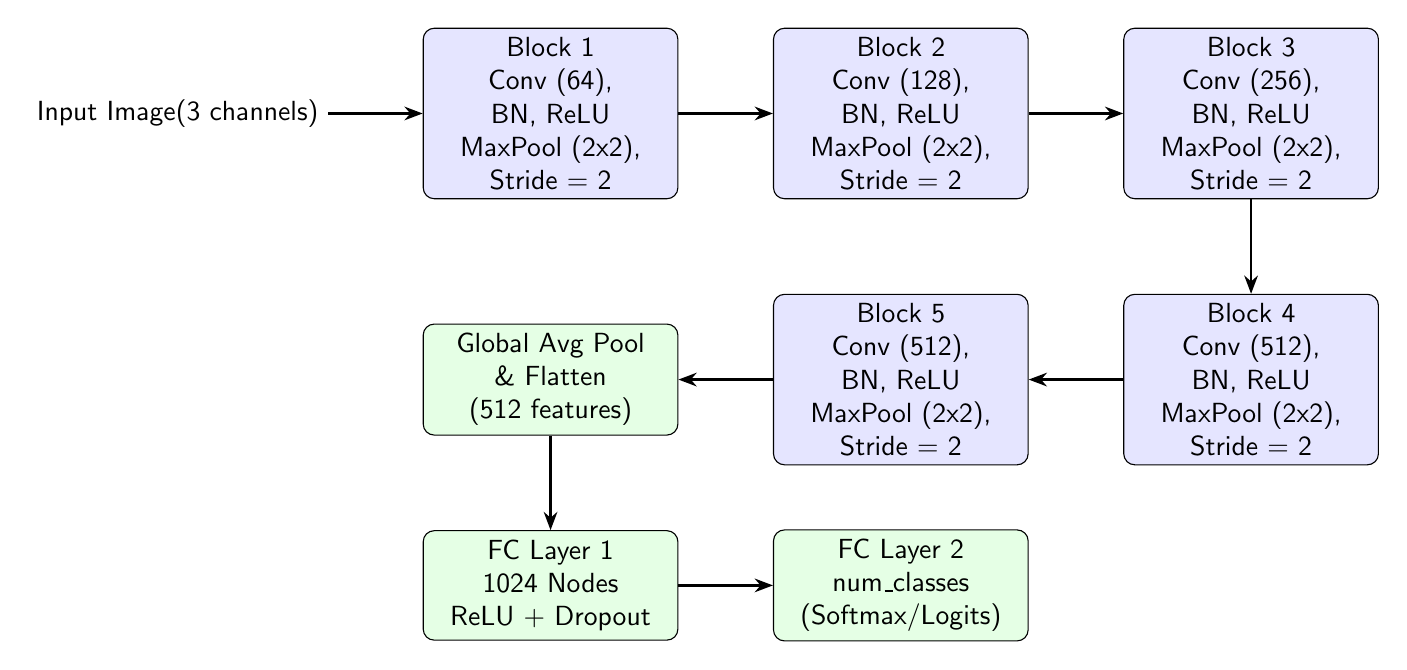
\begin{tikzpicture}[
    node distance=1.2cm,
    start chain=going right,
    block/.style={
        rectangle, 
        draw, 
        fill=blue!10, 
        text width=3cm, 
        align=center, 
        minimum height=1.2cm, 
        rounded corners
    },
    fc/.style={
        rectangle, 
        draw, 
        fill=green!10, 
        text width=3cm, 
        align=center, 
        minimum height=1.2cm, 
        rounded corners
    },
    arrow/.style={-Stealth, thick}
]

% Input
\node (input) [on chain] {Input Image\\(3 channels)};

% Block 1
\node (b1) [block, right=of input] {Block 1\\Conv (64), BN, ReLU\\MaxPool (2x2), Stride = 2};

% Block 2
\node (b2) [block, right=of b1] {Block 2\\Conv (128), BN, ReLU\\MaxPool (2x2), Stride = 2};

% Block 3
\node (b3) [block, right=of b2] {Block 3\\Conv (256), BN, ReLU\\MaxPool (2x2), Stride = 2};

% New row for vertical flow if needed, but we'll continue for clarity
\node (b4) [block, below=of b3] {Block 4\\Conv (512), BN, ReLU\\MaxPool (2x2), Stride = 2};

% Block 5
\node (b5) [block, left=of b4] {Block 5\\Conv (512), BN, ReLU\\MaxPool (2x2), Stride = 2};

% Global Avg Pool + Flatten
\node (gap) [fc, left=of b5] {Global Avg Pool\\\& Flatten\\(512 features)};

% FC 1 + Dropout
\node (fc1) [fc, below=of gap] {FC Layer 1\\1024 Nodes\\ReLU + Dropout};

% FC 2 (Output)
\node (fc2) [fc, right=of fc1] {FC Layer 2\\num\_classes\\(Softmax/Logits)};

% Connections
\draw [arrow] (input) -- (b1);
\draw [arrow] (b1) -- (b2);
\draw [arrow] (b2) -- (b3);
\draw [arrow] (b3) -- (b4);
\draw [arrow] (b4) -- (b5);
\draw [arrow] (b5) -- (gap);
\draw [arrow] (gap) -- (fc1);
\draw [arrow] (fc1) -- (fc2);

\end{tikzpicture}

\caption{CNN Architecture, BN means Batch Normalization, FC means fully connected layer. Global average pooling can be implemented using \texttt{nn.AdaptiveAvgPool2d}. Conv layers have stride of 1 with padding of 1, and maxpool layer has stride of 2.}
\label{fig:cnn}

\end{figure}

\subsection{Deliverables \hfill \textbf{(42 Points)}}
\begin{enumerate}
\item In  \mintinline[bgcolor=faintOrangeYellow]{python}{deepl} subpackage, you already have a module multiclass.py after HW02. There you should define a custom composite layer called \mintinline[bgcolor=faintOrangeYellow]{python}{ConvLayer} corresponding to Block defined in Figure~\ref{fig:cnn}. The layer should be able to take number of input channels and output channels as input argument so that same class can be used to instantiate Block 1 to 5 shown in Figure~\ref{fig:cnn}.


\item Use \mintinline[bgcolor=faintOrangeYellow]{python}{ConvLayer} to create \mintinline[bgcolor=faintOrangeYellow]{python}{ImageNetCNN} class that appropriate put together various layers to construct CNN architecture shown in Fiigure~\ref{fig:cnn}. 

\item You should implement \mintinline[bgcolor=faintOrangeYellow]{python}{CNNTrainer} class similar to how you implemented in Homework 02. However your training function should be able to use training and validation DataLoader as specified above.
Your training function should print epoch number for every tenth batch every epoch, loss and training accuracy, and validation accuracy.

You can exercise some freedom in how you want to implement \mintinline[bgcolor=faintOrangeYellow]{python}{CNNTrainer} but overall structure will be very similar to what you did in Homework 02. You should be able to save trained model as ONNX as well. Do not forget to modify your \mintinline[bgcolor=faintOrangeYellow]{python}{__init__.py}

\item In your scripts folder, create a file called \mintinline[bgcolor=faintOrangeYellow]{python}{imagenet_impl.py} that will be importing your classes defined and perform the following task

\begin{enumerate}
\item Read Imagenet data
\item Perform image transforms and create training and validation dataloader
\item Save an example training and validation image in the script folder. Instantiate your \mintinline[bgcolor=faintOrangeYellow]{python}{ImageNetCNN} and  \mintinline[bgcolor=faintOrangeYellow]{python}{CNNTrainer} classes.
\item You should use cross entropy loss, SGD optimizer with learning rate of 0.01, momentum of 0.9, and weight decay of 1e-4. Use step learning rate scheduler with step size of 30 and gamma value of 0.1.

\item You should be able to write your script in such a way that it should take command line argument such as number of epochs to train, ratio of training dataset and validation dataset to use for training. 

\item At the end of the training, a plot should be saved that should display loss and accuracy as a function of epochs. Commit the plot to the GitHub and provide the file in PDF submission.

\end{enumerate}

\item Write a helping bash script \mintinline[bgcolor=faintOrangeYellow]{python}{imagenet_impl.sh} to execute the training in the background. You don't need to train your image classifier multiple times, but command should have values of number of epochs, and ratio of training dataset and validation dataset to use for training. Supply number of epochs as 10000 at least.

\item Write a Python script called \mintinline[bgcolor=faintOrangeYellow]{python}{imagenet_inference.py} that loads the trained model, take a new image as an argument and predict what class this image belongs to.
Commit the example image, and trained model .onnx to your GitHub. 


\end{enumerate}



\subsection{Questions \hfill \textbf{(2 Each)}}


\begin{enumerate}
\item What is the original number of training samples in the dataset?
\item What is the original number of validation samples in the dataset?

\item How many number of classes are present in the dataset?

\item What is the total number of trainable parameters in your CNN model?

\end{enumerate}


\subsection{Solution}

\begin{enumerate}
\item 1281167
\item 50000
\item 1000
\item 5464040
\end{enumerate}

\section{Cruise Control State Classifier \hfill \textbf{(50 Points)}}
Your goal is create a suprvised classifier to predict the adaptive cruise control status of a car based on the speed data. Valid ACC status are described as:

\begin{tabular}{c l p{7cm}} 
        \toprule
        \textbf{Value} & \textbf{State Name} & \textbf{Description} \\
        \midrule
        0 & \texttt{off} & System Inactive. Main switch is off or ignition cycled. \\
        2 & \texttt{disabled} & Standby. Main switch ON, but no speed set (cancelled). \\
        5 & \texttt{faulted} & System Error. Sensor blocked or hardware failure. \\
        6 & \texttt{enabled} & Active cruising (maintaining speed or following). \\
        10 & \texttt{hold\_waiting\_user\_cmd} & Long Standstill ($>3$s). Holds brakes; requires driver input to move. \\
        11 & \texttt{hold} & Short Standstill ($<3$s). Holds brakes; resumes automatically. \\
        \bottomrule
    \end{tabular}
    
    \vspace{10pt}
    
    

  
Here is the machine learning problem: based on the speed data, determine if ACC is enabled or not. (6 or otherwise).


For that you will create a class called \texttt{ACCNet} in a module \texttt{acc\_classifier.py} in \texttt{deepl} subpackage.


To refer to data for this problem, please to the folder  \texttt{/data/CPE\_487-587/ACCDataset}. It has multiple .csv files. 

You will only need to use those csv files that ends with \texttt{decoded\_wheel\_speed\_fl.csv} along with labels in \texttt{acc\_status.cv}. You will need to binarize the labels as 0 for not ACC and 1 for ACC (which is originally 6 in the above table).

Each of wheel speed fl(fl = front left) csv file names start with a timestamp representing different driving experiment.

In addition, \texttt{decoded\_wheel\_speed\_fl.csv} contains Time column which is in seconds and Message column that has units in km/h that would you need to convert to m/s. Similarly, \texttt{acc\_status.cv} has Time column with values in seconds and Message column that has ACC status. You will need to use any other columns in these two files.

Here is another problem: sampling rate of speed and ACC status are not the same. Hence number of rows in both datasets are not the same. Clearly in that case number of feature samples and number of labels are not the same. In such a case, you can use \textbf{Zero-Order Hold technique} to upsample. See \url{https://en.wikipedia.org/wiki/Zero-order_hold} for more details.


\begin{enumerate}
\item Create a PyTorch Dataset class and PyTorch Dataloader for batch training that takes wheel speed files as input and create multiple feature columns based on historical speed values.

For example, originally, relevant column is Message for \texttt{decoded\_wheel\_speed\_fl.csv}. Call it $v_t$  Your PyTorch Dataset class will take all necessary .csv files as inputs and create a dataset with columns $v_t$, $v_{t-1}$, upto $v_{t-k}$. Choose the value of $k = 10$.

Your neural network will essentialy be an abstraction of the following model:

\begin{align*}
\hat{y_t} = f(\{v_{t-i}\}_{i=0}^k; \Wbf)
\end{align*}

where $\Wbf$ are trainable parameters, and $\yhat$ is the predict cruise control state.


\item Implement a neural network class \texttt{ACCNet} and associated training class. Since ACC state might by highly imbalanced, choose Dice Loss or Focal Tversky Loss as your training metrics. You are free to choose any kind of Neural Network architecture like. You can experiment with different style of architecture like ResNet, FourierNet, etc. or any custom layer for feature engineering, etc. However, you must explain your logic with necessary diagrams or mathematical equations. Custom layer must be implemented as its own class.

There is \textbf{20 Points} bonus for achieve $>90\%$ of validation accuracy.

\item Implement associated implementation script (python and bash scripts) in \texttt{script} folder of your package.

\item You are free to normalize dataset in any way you want use min-max scalar, standard normal scaler, etc.

\item Use most available GPU for training using GPU device selection method specified in the previous problem.

\item Save the trained model as ONNX along with normalizing coefficients to test with an unseen dataset. Commit ONNX file to your GitHub.


\end{enumerate}

\end{document}
